\section*{一、预习报告}

\subsection*{1. 实验综述}

通过预习，我了解到日光灯电路是典型的感性负载。本实验先组装日光灯电路，再测量并联不同电容时的电压、电流和功率，研究提高功率因数（power factor）的方法。

日光灯由灯管、镇流器和启辉器组成。启动时，启辉器先接通使灯丝预热，随后断开，镇流器产生自感高压，使灯管内气体放电，激发荧光粉发光。正常工作后，启辉器保持断开，镇流器起限流作用。

\begin{figure}[H]\centering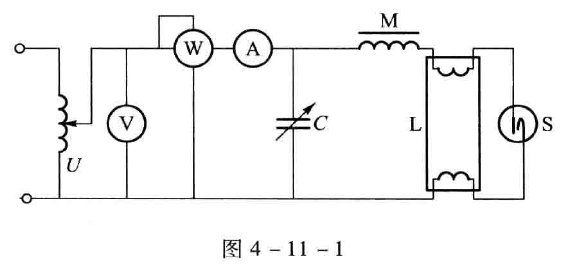
\includegraphics[width=7cm]{assets/power-circuit.png}\caption{日光灯及并联电容补偿原理图（教材图 4-11-1）}\end{figure}

图中 $M$、$L$、$S$ 分别为镇流器、灯管和启辉器，$C$ 为补偿电容。按教材的正弦交流模型，电路有功功率为

\[
P=UI\cos\varphi,\qquad \cos\varphi=\frac{P}{UI},
\]

其中 $U$、$I$ 为电压和电流的有效值，$\varphi$ 为相位差。感性负载的电流滞后于电压；并联适当电容后，电容电流补偿滞后分量，使总电流减小、功率因数提高，从而降低线路损耗。不过，电容过大时会出现过补偿，总电流重新增大，功率因数反而下降。

由于标称数据可能不准确，我先打开 LCR 电表，切换至电容档，重新测量各电容的实际电容值。接着使用变频交流电源，将输出电压调至 $220\,\mathrm{V}$，频率设在 $45\sim55\,\mathrm{Hz}$ 范围内。随后测量未接电容时的 $U$、$I$、$P$，再保持供电电压和频率一致，按教材依次接入 $1\sim7\,\mu\mathrm{F}$ 的电容并记录读数。随后计算各组功率因数，绘制 $\cos\varphi-C$ 曲线，找出已测档位中功率因数最大时的电容值，并比较补偿前后电流和功率的变化。

\subsection*{2. 实验目的}

\begin{enumerate}
\item 了解日光灯的工作原理，掌握电路的组装方法。
\item 学习交流电压表、电流表和功率表的使用，测量电路功率因数。
\item 理解并联电容提高功率因数的原理，观察过补偿现象。

\end{enumerate}
\subsection*{3. 实验重点与难点}

\begin{enumerate}
\item 正确连接功率表的电流、电压线圈及同名端，分别核对量程，避免过载。
\item 比较不同电容时保持电压和频率一致，待灯管和示数稳定后读数；注意交流电流应按相量相加，不能直接相加有效值。
\item 接线须经教师检查后才能通电。开启时从左到右依次打开开关，关闭时从右到左依次关闭开关。严禁带电接线、改线或更换电容，操作前须断电并按要求使电容安全放电。
\end{enumerate}
